\documentclass[12pt, letterpage]{article}
\usepackage{graphicx}
\usepackage{float}
\usepackage{sectsty}

\title{EAS 4/587 – Data Intensive Computing\\Phase 1 Report}
\author{
    Kumar Priyansh \\
    \footnotesize UBIT Name: kumarpri
    \and Ritu Dimri\\
    \footnotesize UBIT Name: ritudimr
}
\date{}
\sloppy
\graphicspath{{../images/}}

\begin{document}
\maketitle

\section{Motivation \& Problem Statement}

\subsection{Motivation}
\begin{itemize}
    \item Reddit is a social media website where users can post links to articles, images, videos, etc.\ and other users can comment on them. Authors of the posts, generally look to drive maximum engagement from their posts.
    \item Unlike other social media websites, Reddit has a unique feature of upvoting and downvoting the posts. Also, since the posts are publicly visible, factors like the time of posting, the number of upvotes, the number of comments, etc.\ matter a lot.
    \item Since there are a lot of posts being made every minute, significant posts can get lost in the crowd. Also, the posts that are made at a particular time of the day, may not be visible to the users who are active at a different time of the day.
\end{itemize}

\subsection{Problem Statement}
\begin{itemize}
    \item Fetch the data using the Reddit Developer API from different programming related subreddits (communities). Since, there are a lot of subreddits on Reddit; we will keep the scope of the project limited.
    \item Analyze the data and find relevant insights after cleaning and preprocessing the data.
    \item Build a model to predict the engagement a post will likely receive, given the time of posting, the number of upvotes, the number of comments, and other factors.
\end{itemize}

\section{Data Collection}

The data was collected from the Reddit Developer API\footnote{https://www.reddit.com/dev/api/}. The API provides access to the data of the posts made on Reddit. The data was collected from the following subreddits: 

\texttt{python},
\texttt{datascience}, \texttt{javascript},
\texttt{linux}, \texttt{opensource}, \texttt{node},
\texttt{programming}, \texttt{computerscience},
\texttt{webdev}, \texttt{statistics}, \texttt{machinelearning}, \texttt{compsci}, \texttt{java}, \texttt{rust}, \texttt{typescript}.

\section{Data Cleaning \& Preprocessing}

\textbf{Note:} Since the data is coming from a live API, the data is not static. Hence, the plots and the results may vary from the ones shown in the report. \\

After collecting the data, we got more than 15,700 rows and 118 columns. The data was cleaned and preprocessed to remove the unnecessary columns and to make the data more readable. The data was cleaned and preprocessed using the following steps:

\begin{enumerate}
    \item \textbf{Dropping Saturated Columns}: Saturated columns are the columns that have a single value for all the rows. These columns do not provide any useful information and hence, they were dropped.
    \item \textbf{Fixing Data Types}: Some columns can have incorrect data type when converted into a Pandas DataFrame. All data was converted to \texttt{string} type, except numeric (\texttt{int} \& \texttt{float}) and \texttt{boolean} columns. Some boolean colums like \texttt{distinguished} and \texttt{author\_premium}  required forced type conversion to \texttt{boolean} type.
    \item \textbf{Drop Duplicates}: Sometimes, the same post is copied and pasted in multiple subreddits. These posts are duplicates and hence, they were dropped, keeping only one copy of the post.
    \item \textbf{Check for Missing and Null Values}: The data was checked for missing and null values. After the above steps, there were no missing or null values in the data.
    \item \textbf{Handling Flairs}: Flairs are the tags that are assigned to the posts. They are used to categorize the posts. For example, a post can be tagged as \texttt{help}, \texttt{discussion}, \texttt{news}, etc.\ Only the relevant flair columns were kept. The flairs might also contain emojis, which were also removed in a later step.
    \item \textbf{Handling Deleted Posts \& Posts by Deleted Users}: Posts that were deleted by the author or the moderators were removed from the data. Also, posts by deleted users were removed.
    \item \textbf{Handling Polls}: Polls are posts that are used to collect votes from the users. These posts were removed from the data as they do not provide any useful information for text analysis.
    \item \textbf{Dropping Unnecessary Columns}: Some columns were dropped as they were not relevant for the analysis. For example, columns like \texttt{thumbnail\_height} and \texttt{thumbnail\_width} were dropped as they do not provide any useful information.
    \item \textbf{Lowecasing Text Columns}: All text columns were converted to lowercase.
    \item \textbf{Removing HTML Entities, Escape Characters and URLs}: HTML entities, escape characters and URLs were removed from the text columns.
    \item \textbf{Removing Punctuations, Numbers and Emojis}: Punctuations, numbers and emojis were removed from the text columns.
    \item \textbf{Removing Stopwords \& Contractions}: Stopwords and contractions were removed from the text columns.
    \item \textbf{Lemmatization \& Stemming}: Lemmatization and stemming were performed on the text columns to reduce the words to their root form.
\end{enumerate}

\pagebreak
\section{Expolaratory Data Analysis}

After cleaning and preprocessing the data, we were left with around 8,000+ rows and 28 columns. The data was analyzed to find relevant insights. The data was analyzed using the following steps: 

\subsection*{Number of Posts Fetched per Subreddit}
\begin{figure}[H]
    \centering
    \includegraphics[width=0.8\textwidth]{num_posts_per_subreddit.png}
    \caption{Number of Posts per Subreddit}
    \label{fig:posts_per_subreddit}
\end{figure}

\subsection*{Number of Subscribers per Subreddit}
\begin{figure}[H]
    \centering
    \includegraphics[width=0.8\textwidth]{num_subscribers_per_subreddit.png}
    \caption{Number of Subscribers per Subreddit}
    \label{fig:subscribers_per_subreddit}
\end{figure}

\subsection*{Number of Authors who post in multiple subreddits}
\begin{figure}[H]
    \centering
    \includegraphics[width=0.8\textwidth]{num_authors_multiple_subreddit.png}
    \caption{Number of Authors who post in multiple subreddits}
    \label{fig:authors_per_subreddit}
\end{figure}

From the above figure, it seems like most of the authors post in only one subreddit.

\subsection*{Does posting in multiple subreddits drives more upvotes?}
\begin{figure}[H]
    \centering
    \includegraphics[width=0.8\textwidth]{post_multiple.png}
    \caption{Does posting in multiple subreddits drives more upvotes?}
    \label{fig:upvotes_per_subreddit}
\end{figure}

From the above figure, it seems like authors who post in multiple subreddits get more upvotes, generally.

\subsection*{History of posts per day per subreddit (Past 6 months)}

\begin{figure}[H]
    \centering
    \includegraphics[width=1\textwidth]{num_posts_per_day_per_subreddit.png}
    \caption{History of posts per day per subreddit}
    \label{fig:history_posts_per_day}
\end{figure}

From the above figure, it seems like the number of posts per day is increasing for most of the subreddits.

\subsection*{Number of posts per subreddit, categorized by days of the week}

\begin{figure}[H]
    \centering
    \includegraphics[width=1\textwidth]{num_posts_per_day_per_subreddit_bar.png}
    \caption{Number of posts per day per subreddit}
    \label{fig:posts_per_day}
\end{figure}

The above figure presents total number of posts per subreddit, categorized by the days of the week.

\subsection*{Top 10 Authors Per Subreddit}

\begin{figure}[H]
    \centering
    \includegraphics[width=0.95\textwidth]{author_rank.png}
    \caption{Top 10 Authors Per Subreddit}
    \label{fig:top_authors_per_subreddit}
\end{figure}

The above plot was generated by creating an author ranking system. The authors were then sorted in descending order of their rank. The top 10 authors were then plotted. The ranking system uses the following simple formula to rank the authors:

\begin{equation}
    \textnormal{Rank} = \textnormal{Post Score} \times \textnormal{Upvote Ratio} + \textnormal{Number of Comments}
\end{equation}

\subsection*{Finding the best time to post on each subreddit}

\begin{figure}[H]
    \centering
    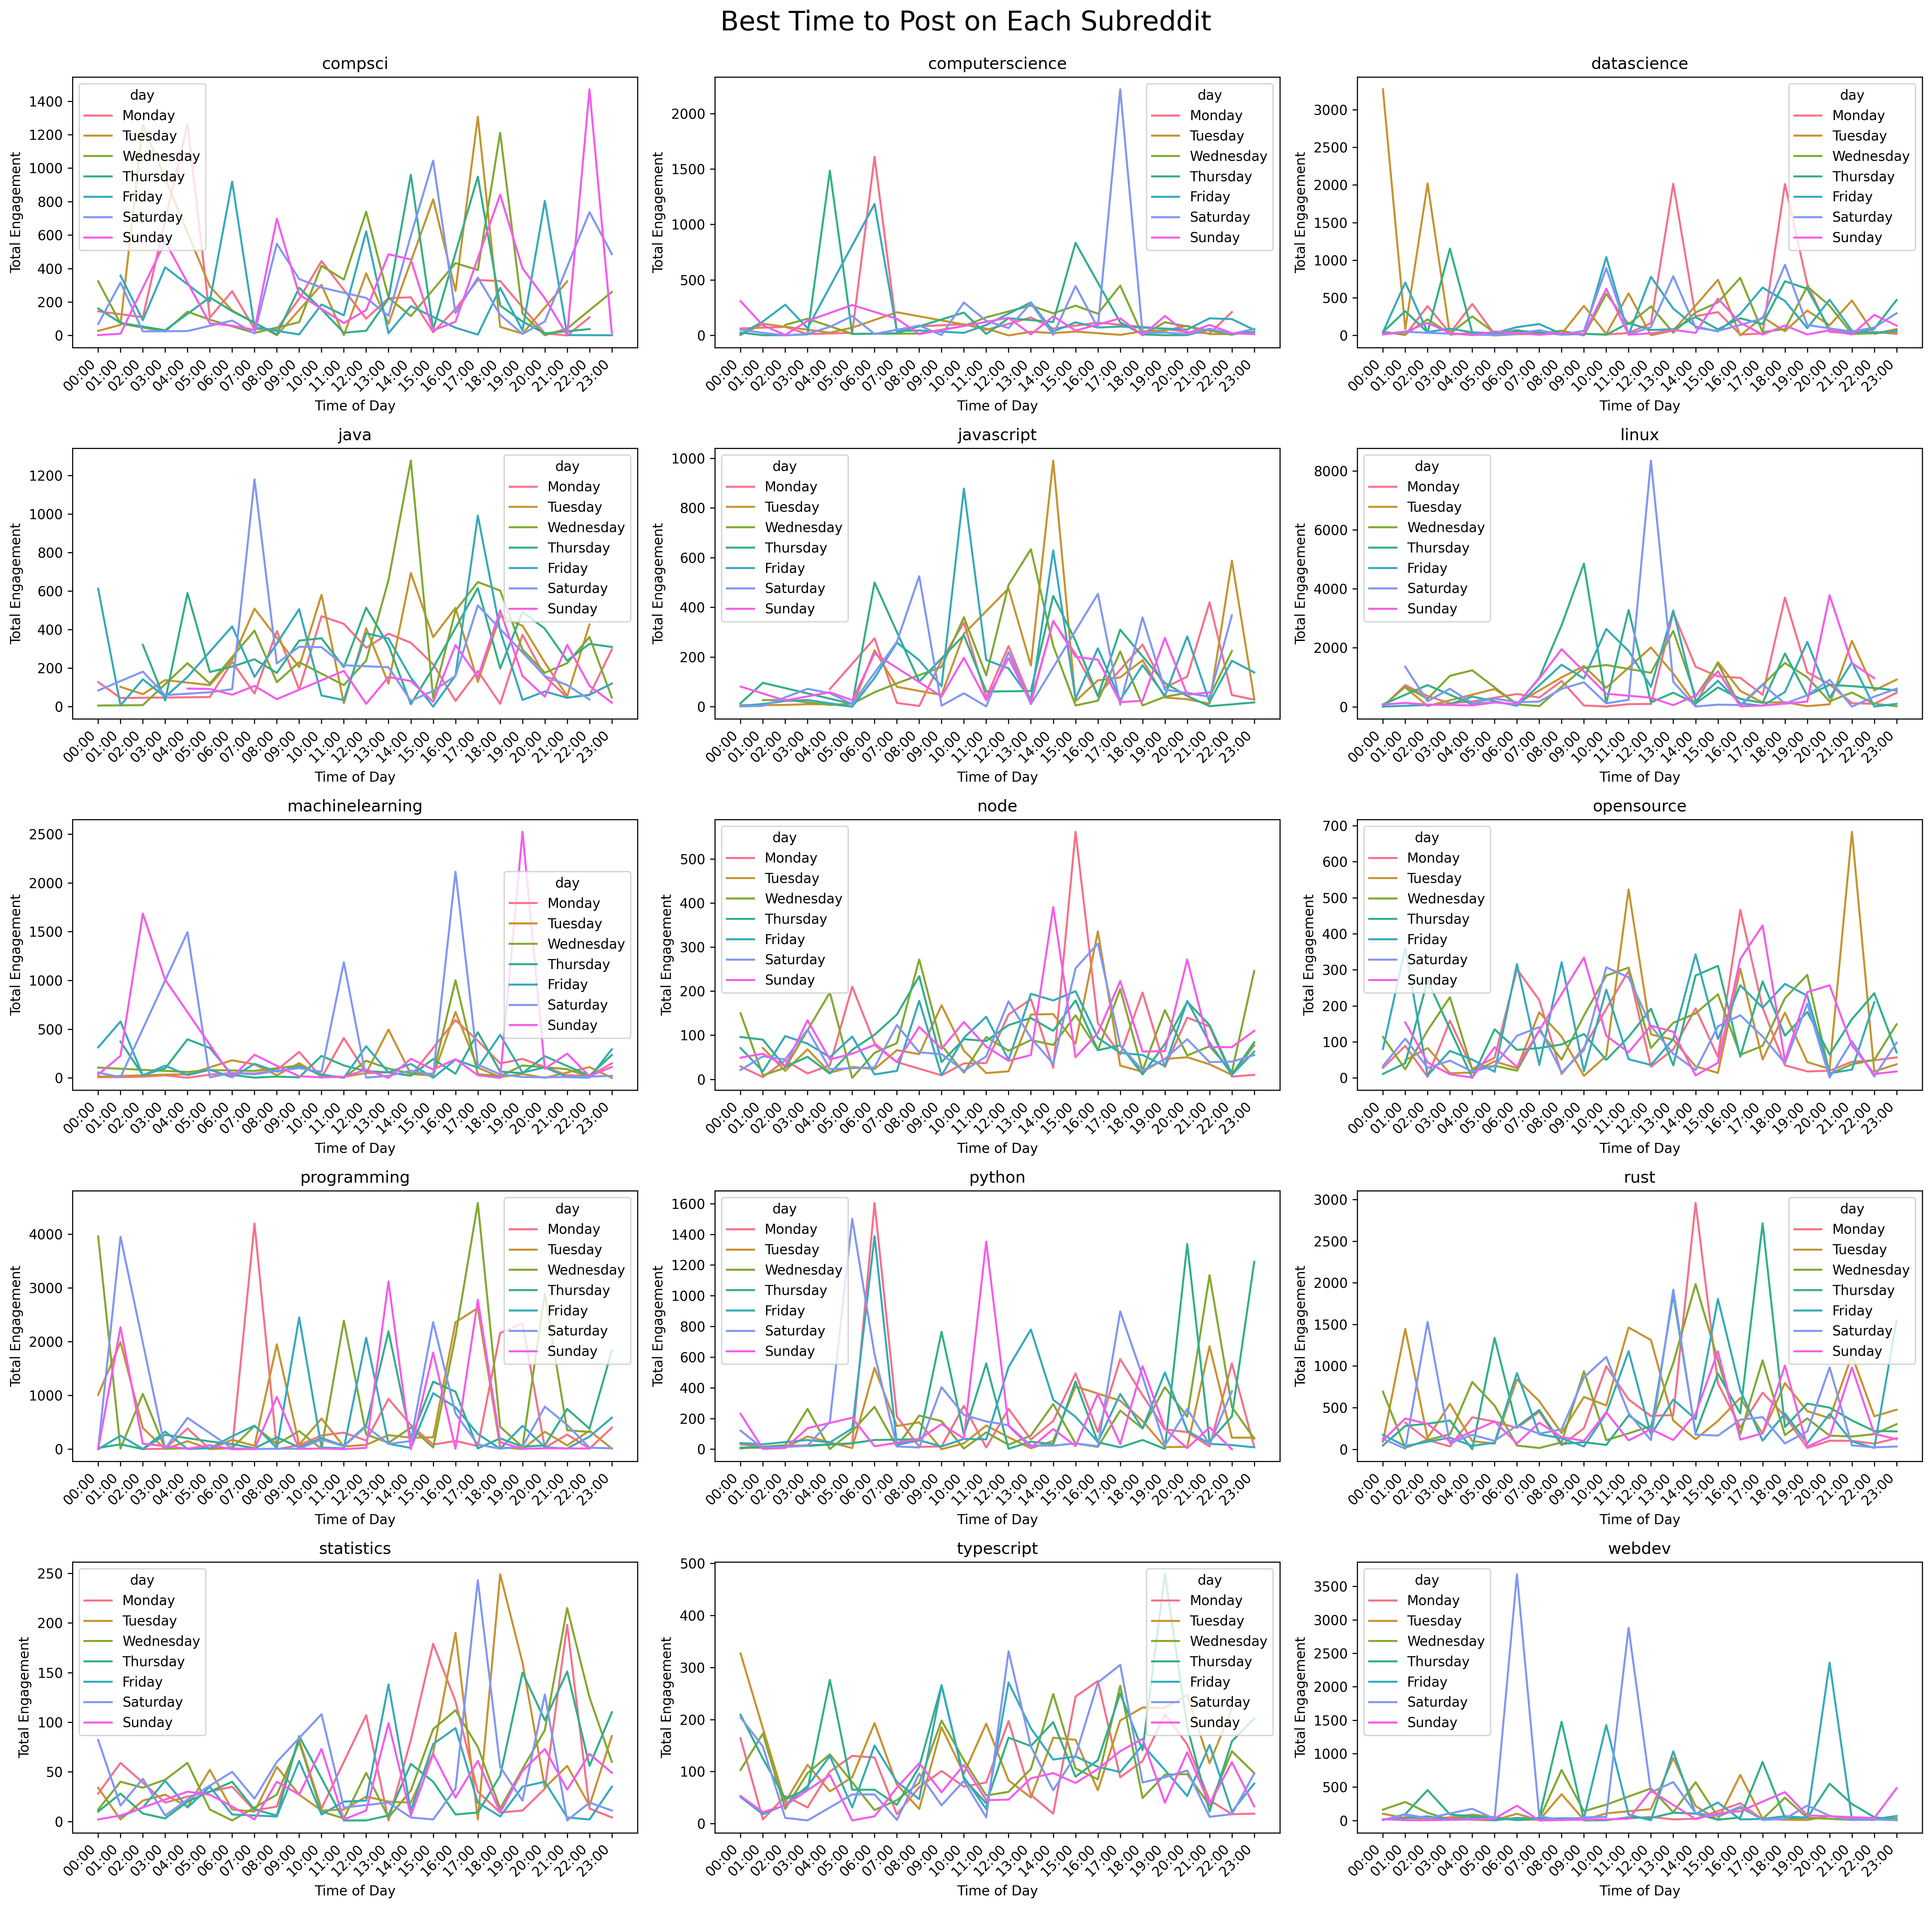
\includegraphics[width=1\textwidth]{best_time.png}
    \caption{Best Time to Post on each Subreddit}
    \label{fig:best_time_to_post}
\end{figure}

The above plot was generated by finding the total hourly engagement on each subreddit, categorized by each day. It seems like the best time to post on each subreddit is different and there happens to be a peak in the engagement at different times of the day.

\subsection*{Scatterplot of the scores vs number of comments in each subreddit}

\begin{figure}[H]
    \centering
    \includegraphics[width=1\textwidth]{scatterplot_scores.png}
    \caption{Scatterplot of the scores vs number of comments in each subreddit}
    \label{fig:score_vs_comments}
\end{figure}

The above plot was generated by plotting the scores vs number of comments in each subreddit. It seems like there is a positive correlation between the scores and the number of comments, except for some controversial posts, which tend to get more comments than the scores.

\subsection*{\% of Authors opted to receive comment notifications per Subreddit}

\begin{figure}[H]
    \centering
    \includegraphics[width=1\textwidth]{pie_comments.png}
    \caption{\% of Authors opted to receive comment notifications per Subreddit}
    \label{fig:comment_notifications}
\end{figure}

The above plot was generated by finding the percentage of authors who opted to receive comment notifications in each subreddit. It seems like most of the authors opted to receive comment notifications.

\subsection*{Total Awards Received vs Upvotes per Subreddit}

\begin{figure}[H]
    \centering
    \includegraphics[width=1\textwidth]{awards_per_subreddit.png}
    \caption{Total Awards Received vs Upvotes per Subreddit}
    \label{fig:awards_vs_upvotes}
\end{figure}

Good posts are usually awarded with ``awards". The above plot was generated by plotting the total awards received vs upvotes in each subreddit. It seems like there is a positive correlation between the total awards received and the upvotes.

\subsection*{Boxplot of the scores in each subreddit}

\begin{figure}[H]
    \centering
    \includegraphics[width=1\textwidth]{boxplot_scores.png}
    \caption{Boxplot of the scores in each subreddit}
    \label{fig:boxplot}
\end{figure}

The above plot was generated by plotting the boxplot of the scores in each subreddit. It seems like most of the scores are concentrated in the lower range, except for a few outliers – they are the posts that went viral. It means that most of the posts are not very popular.

\end{document}